\chapter{Experimental Methodology} 

Our initial goal was to implement a couple of algorithms as baseline for
experiments outside of the scope of this work. Ideally, those algorithms would
have also helped us finding any ``low-hanging fruits'' to properly start
tackling the game as a whole. In addition to implementing those algorithms, we
also designed a few automatic tests to check the validity of the game state
information in known maps.  

\section{Test Task}

\section{RL Algorithms}

At the start of the project we decided that by the end of it we would have had a
classic model-free RL algorithm to test an MDP-like setting and the newer DQN, a
deep reinforcement learning algorithm, to test learning policies purely from the
visual input. 

\subsection{Q-learning}

The choice of Q-learning as the test model-free algorithm was relatively
straightforward: Q-learning is one of the most popular and powerful model-free
RL algorithms, and it represents the foundation of many other reinforcement
learning algorithms. Given a standard MDP in the form of a tuple $(S, A, T, R)$
where $S$ is the state space, $A$ is the action space, $T(s, s')$ is the
transition probability distribution of moving from state $s$ to state $s'$, and
$R$ is the immediate reward received when moving from state $s$ to state $s'$,
Q-learning allows to iteratively find a policy that maximises the expected total
reward in a trial by learning from experience gained by some policy (as opposed
to on-policy reinforcement learning where the samples are  to the
policy being learnt).

In particular, the algorithms works by updating an action-value function $Q(s,
a)$ using an $\epsilon$-greedy policy to gain new samples. Given a learning rate
$\alpha$ and a discount factor $\gamma$,


\begin{equation}
  Q(s_t, a_t) \leftarrow Q(s_t, a_t) +
  \alpha \left[ r_{t+1} + \gamma \max_a Q(s_{t+1}, a) - Q(s_t, a_t) \right].
\label{eq:ql}
\end{equation}

The agent policy in the evaluation phase then becomes

\begin{equation}
  \pi(s, a) = \operatornamewithlimits{argmax}_a Q(s, a).
\label{eq:ql2}
\end{equation}

It has been proved that this policy converges to the optimal policy $\pi*$ given
enough samples from all state-action pairs. % TODO how?

The Q function can be represented as a table of values (a simple array) or can
be approximated using a function approximator, however a lot of literature has
highlighted difficulties in making Q-learning (and other model-free RL
algorithms) converge when the action-value function is approximated
\citep{Baird_1997}. In some cases researched managed to converge the algorithms,
but obtained significantly degraded policies \citep{bertsekas_1996_tetris,
  waver_and_baxter_1999, boyan_and_moore_1995}.

\subsubsection{Task dependent state representation}

Providing a state representation for quickly testing the whole system ended up
resulting in a far more challenging problem than initially estimated. To be able
to extensively test the symbolic game state data being sent by the client we
wanted to obtain a useful state representation without having to use a black-box
function approximator such as an artificial neural network. Using a neural
network would have made it very hard to do automatic testings. Moreover we
wanted to check and explore how difficult it would have been to use standard RL
techniques on StarCraft's large state space.

\begin{figure}[h]
    \centering
    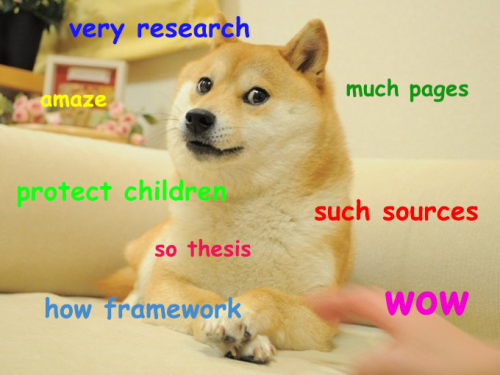
\includegraphics[width=0.9\textwidth]{placeholder}
    \caption{Example of a state in our test domain.}
    \label{fig:sample_state}
\end{figure}

Figure \ref{fig:sample_state} shows a sample of the game state data in our
domain. We can see that it is difficult to represent such a representation in an
array because the data increases with the number of units. To create a
representation that we can use in a tabular fashion we must approximate the
state in some way.

\begin{figure}[h]
    \centering
    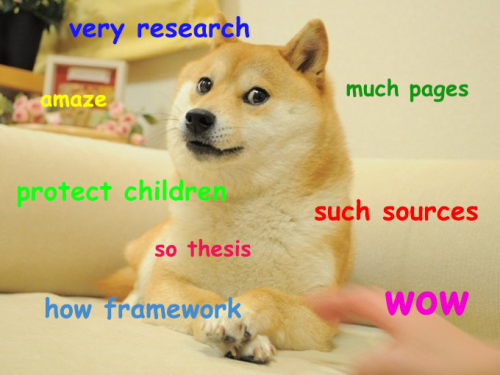
\includegraphics[width=0.9\textwidth]{placeholder}
    \caption{Discretisation of state based on units health points.}
    \label{fig:discrete_state}
\end{figure}

We chose to approximate the state by discretise a potential function
\citep{diebelthrun} based on the health points of in-game units relative to a
particular selected allied unit (Figure \ref{fig:discrete_state}). This was
achieved by taking a particular unit as reference, filtering out everything
lying outside of the visible pixel radius, splitting then the obtained space
into a variable amount of slices. The value of each slice was then calculated by
obtaining the sum of all health ``value'' assigned to each unit within a space.
Given slice $p$ and $U_p$ units, the slice value $SV(p)$ is computed as

\begin{equation}
  \begin{aligned}
    SV(p, \beta) = & 
    \begin{cases}
      \sum_{u \in U_p}{UV(u)} & \text{if } \sum_{u \in U_p}{UV(u)} < \beta \\
      \beta & otherwise\\
    \end{cases}, \\ \text{where } 
    UH(u) = &
    \begin{cases}
      1 & \text{if } \text{health}_u < 50\%\\
      2 & otherwise \\
    \end{cases} 
  \end{aligned}
\end{equation}

We created a pair of partitions for each class of unit representing allied units
and enemy units, and added to the top the value of the reference unit health,
ending up with a relatively large tensor as our index for our action-value
function (Figure \ref{fig:array_state}).

\begin{figure}[h]
    \centering
    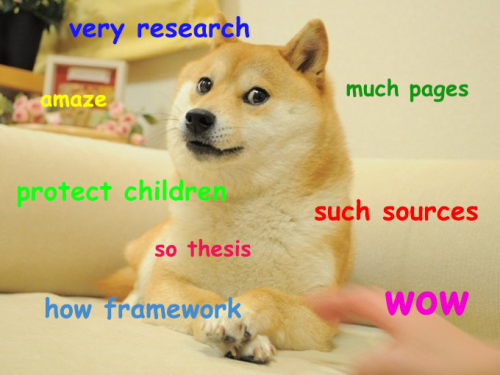
\includegraphics[width=0.9\textwidth]{placeholder}
    \caption{Mapping from slices to index tensor.}
    \label{fig:array_state}
\end{figure}

We could have also used a tile-coding technique\citep{stone_sutton_keepaway} to
stack multiple partitions of the same space (but different starting points) and
increase the generality of our state representation, but we didn't have the time
to finish its implementation.

This final technique is reasonable (as tests later confirmed) for our task, but
it wouldn't necessarily lend itself well to other scenarios. Our representation
for instance entirely lacks information about upgrades, bullets, visibility of
the map and state of the fog of war. It must be noted that with this
representation the problem becomes more complex than a standard MDP, as we are
not using the entirety of the available state information by filtering
everything outside of the image radius. We could have also used an observation
window to solve the partial observability problem, but we hypothesised that we
would obtain a good enough (but almost certainly suboptimal) policy in any case.

% TODO add missing sliding state windows.

\subsection{Deep Q-learning}

Our work is partially motivated by recent advances in work that uses non-linear
function approximators for reinforcement learning. DeepMind's Deep Q-Network has
become one of the most popular variants of deep reinforcement learning, a
``new'' branch of reinforcement learning research that uses multi-layer ``deep''
neural networks (and other deep learning techniques) as functions approximators
to aid the decision-making process. They released their implementation together
with their Nature paper, both of which we used as a reference to develop a
version of DQN compatible with our interface.

Our Deep Q-learning algorithm works by approximating the action-value function
$Q(s, a)$ with a Convolutional Neural Network. The network takes as input the
state (in our case, the screen image) and returns an array of values of the same
size as the number of actions available. The $\epsilon$-greedy policy then
chooses the action whose output value is highest, or occasionally another random
action.

\begin{figure}[h]
    \centering
    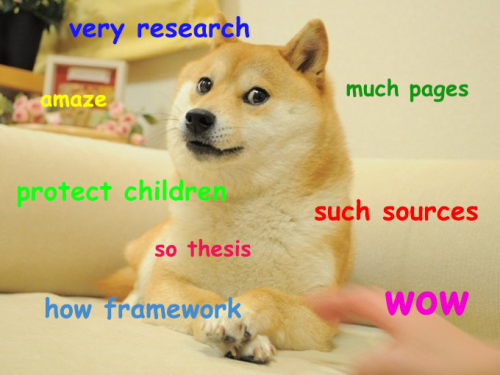
\includegraphics[width=0.9\textwidth]{placeholder}
    \caption{Deep Q-learning visualised.}
    \label{fig:dqn}
\end{figure}

If we consider the problem in a supervised learning fashion and imagine our
input dataset as just being generated by the interaction with the environment,
this problem then essentially becomes building a regression model with a neural
network trained using stochastic gradient descent algorithm that uses the
Q-learning update (Equation \ref{eq:ql}) as the loss function.

% TODO maybe put algorithm in here

Similarly to \cite{mnih_et_al}, our algorithms records all the tuples containing
the experience of the agent, keeps track of the newest ones using a circular
buffer, and samples from the buffer whenever the update step is called. This
functionality is called \textbf{Experience Replay} and removes the correlation
in the sequential observations, reducing the forgetting rate in the network. To
again reduce the correlation, temporal-difference error uses a copy of the
Q-network that is saved every now and then. Finally in addition we added a
maximum cap value to the temporal-difference error to reduce big outliers and
stop the weights from changing too much when those appear.

% TODO check paper for above, in case it needs rewriting.

\subsection{Multi-unit RL}

In the previous two sections we purposely avoided discussing a huge issue with
our algorithms: by default they assume that the controlled agent is one, while
instead in StarCraft the player usually has to independently control multiple
units.

We didn't manage to find the time to implement a multi-agent reinforcement
learning algorithm, so we decide to handle multi-unit scenarios in both
Q-learning and Deep Q-learning. 

The most effective way to coherently allow our algorithms to use multiple units
at the same time would have been to parametrise the actions by units ids, but
the actions space would then quickly explode. Additionally both our algorithms
(or at least their implementations) require the action number to be known
a priori.

Instead we came up with a system to optimise the execution of each unit action
by parallelising the decision process using the duration of the commanded
primitive as a time buffer.

\begin{figure}[h]
    \centering
    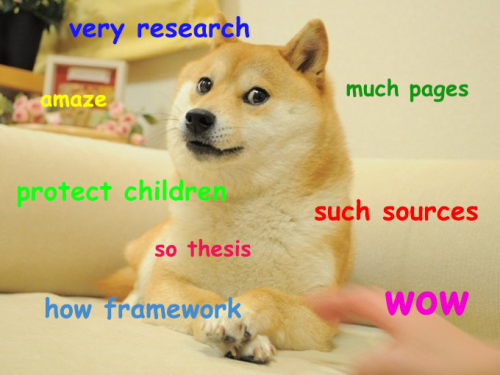
\includegraphics[width=0.9\textwidth]{placeholder}
    \caption{Visualisation of the parallel system for Q-learning.}
    \label{fig:parallelq}
\end{figure}

Q-learning was the easy to adapt, as the only required change to the algorithm
was to generate the state with respective to selected units and send the
required actions to the client (Figure \ref{fig:parallelq}). Deep Q-learning was
harder to adapt because we had to take into account the visual window state. In
particular, to minimise the pixel variance we had to order the client to
position the window viewpoint on top of the unit to always keep it at the center
of the screen (Figure \ref{fig:paralleldq}).

\begin{figure}[h]
    \centering
    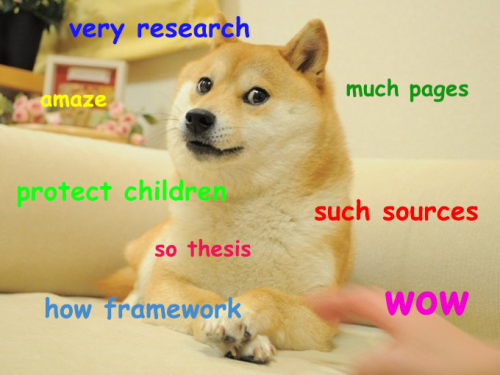
\includegraphics[width=0.9\textwidth]{placeholder}
    \caption{Visualisation of the parallel system for Deep Q-learning.}
    \label{fig:paralleldq}
\end{figure}

This had the additional unexpected consequence of further randomising our
experiments, therefore allowing us to explore the state space much more quickly.
Unfortunately it also meant that the agent would not have any information about
the effect of its previous units' action choices over its future observations,
making the behaviour of allied units somewhat correlated.

% TODO maybe add that we had no way to check for this.

\section{Hardware Setup}

TODO.